\documentclass[border={0.1cm 0.1cm 0.1cm 0.1cm}]{standalone}  %E,S,W,N

\usepackage{amssymb}
\usepackage{amsmath}
\usepackage{tikz}

\begin{document}
	
	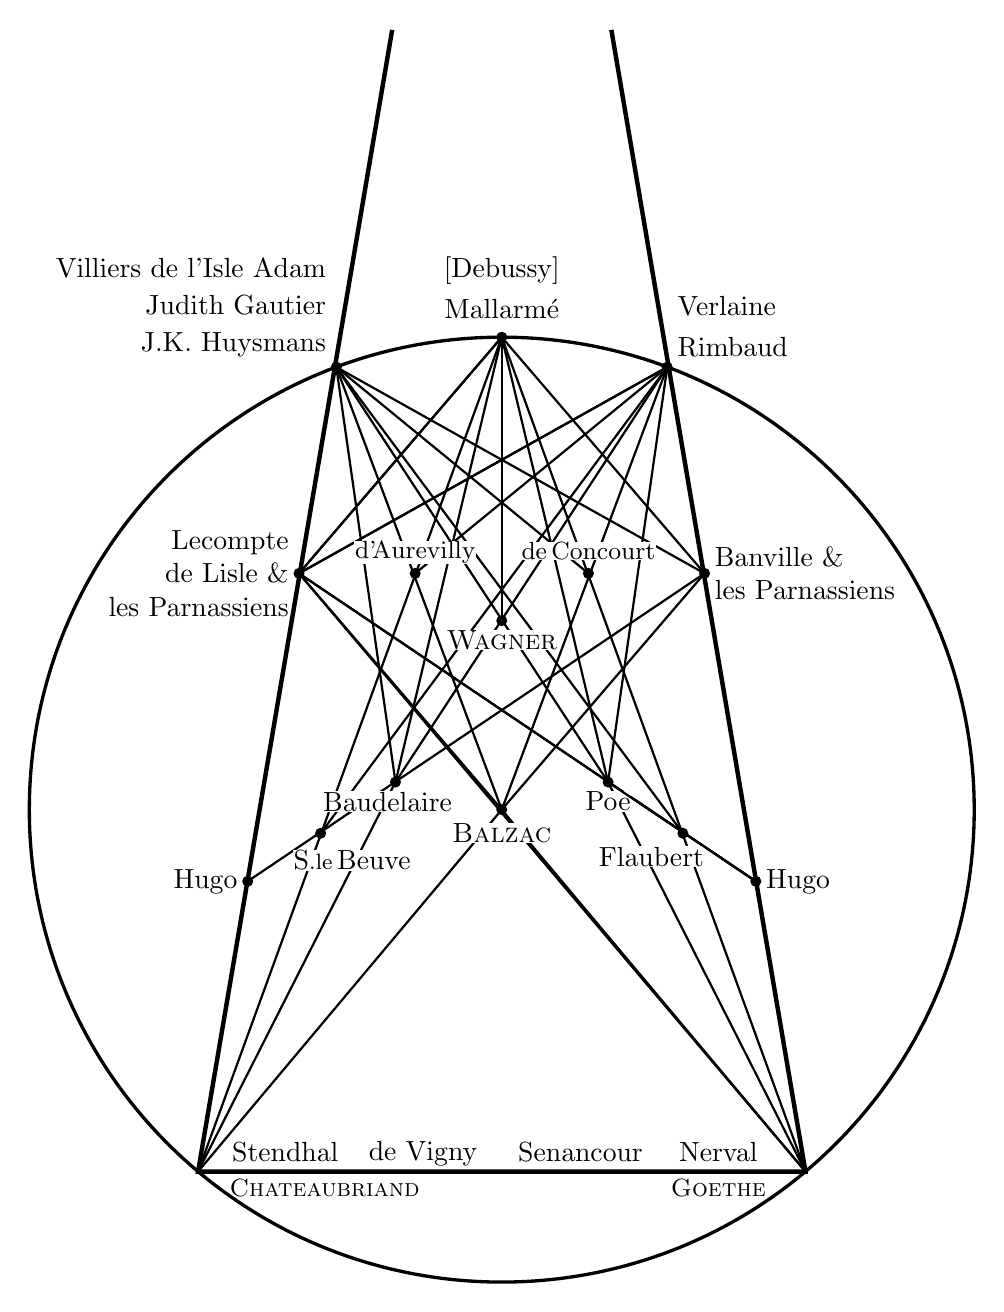
\begin{tikzpicture}[thick]
	%MAIN CIRCLE
	\draw[very thick] (0,0) circle (6cm);
	\draw[ultra thick] ({10*cos(98)},{10*sin(98)})--({6*cos(230)},{6*sin(230)})-- ({6*cos(310)},{6*sin(310)})--({10*cos(82)},{10*sin(82)});
	
	%AUTHORS
	\coordinate (Stendhal) at ({6*cos(230)},{6*sin(230)});
	\coordinate (Nerval) at ({6*cos(310)},{6*sin(310)});
	\coordinate (Adam) at ({6*cos(90+20.5)},{6*sin(90+20.5)});
	\coordinate (Mallarme) at ({6*cos(90)},{6*sin(90)});
	\coordinate (Verlaine) at ({6*cos(90-20.5)},{6*sin(90-20.5)});
	\coordinate (HugoL) at ({6*cos(230)-0.3*6*cos(90+20.5)},{6*sin(230)+2+0.3*6*sin(90+20.5)});
	\coordinate (HugoR) at ({6*cos(310)-0.3*6*cos(90-20.5)},{6*sin(310)+2+0.3*6*sin(90-20.5)});
	\coordinate (Wagner) at (0,2.4);
	\coordinate (Baudelaire) at (-1.35,0.35);
	\coordinate (Poe) at (1.35,0.35);
	\coordinate (Balzac) at (0,0);
	\coordinate (deLisle) at (-2.575,3);
	\coordinate (Banville) at (2.575,3);
	\coordinate (leBeuve) at (-2.3,-0.3);
	\coordinate (Flaubert) at (2.3,-0.3);
	%
	\coordinate (dAurevilly) at (-1.1,3);
	\coordinate (deConcourt) at (1.1,3);
	
	%LINES
	\foreach \w in {Mallarme,Verlaine,HugoR,Nerval} \draw (deLisle)--(\w); %de Lisle
	\foreach \w in {deLisle,Stendhal,Baudelaire,Wagner,Poe,Nerval,Banville} \draw (Mallarme)--(\w); 
	\foreach \w in {Baudelaire,Balzac,Poe,Flaubert,deConcourt,Banville} \draw (Adam)--(\w); 
	\foreach \w in {deLisle,dAurevilly,leBeuve,Baudelaire,Balzac,Poe} \draw (Verlaine)--(\w); 
	\foreach \w in {Baudelaire,Balzac} \draw (Stendhal)--(\w); 
	\foreach \w in {Poe,Balzac} \draw (Nerval)--(\w); 
	\foreach \w in {HugoR,Balzac} \draw (deLisle)--(\w);
	\foreach \w in {HugoL,Balzac} \draw (Banville)--(\w); 
	
	%CIRCLES / LABELS
	\fill (Balzac) circle (2pt) node[below,fill=white,inner sep=0.1mm,yshift=-1.5mm] {\scshape Balzac};
	\fill (Adam) circle (2pt) node[align=right,above left] {Villiers de l'Isle Adam \\[0.5mm] Judith Gautier \\[0.5mm] J.K. Huysmans};
	\fill (Verlaine) circle (2pt) node[align=left,above right] {Verlaine \\[1mm] Rimbaud};
	\fill (Wagner) circle (2pt) node[below,fill=white,inner sep=0.1mm,yshift=-1mm] {\scshape Wagner};
	\fill (dAurevilly) circle (2pt) node[above,fill=white,inner sep=0.1mm,yshift=1mm] {\small d'$\!$Aurevilly};
	\fill (deConcourt) circle (2pt) node[above,fill=white,inner sep=0.1mm,yshift=1.5mm] {\small de$\,$Concourt};
	\fill (Mallarme) circle (2pt) node[align=center,above,yshift=1mm] {[Debussy] \\[1mm] Mallarm\'{e}};
	\fill (Baudelaire) circle (2pt) node[below,fill=white,inner sep=0.1mm,yshift=-1mm,xshift=-1mm] {Baudelaire};
	\fill (Poe) circle (2pt) node[below,fill=white,inner sep=0.1mm,yshift=-1mm] {Poe};
	\fill (deLisle) circle (2pt) node[align=right,left] {Lecompte \\ de Lisle \& \\ les Parnassiens};
	\fill (Banville) circle (2pt) node[align=left,right] {Banville \& \\ les Parnassiens};
	\fill (leBeuve) circle (2pt) node[below,fill=white,inner sep=0.1mm,yshift=-2mm,xshift=4mm] {S{\footnotesize.le}$\,$Beuve};
	\fill (Flaubert) circle (2pt) node[below,fill=white,inner sep=0.1mm,yshift=-1.5mm,xshift=-4mm] {Flaubert};
	\fill (HugoL) circle (2pt) node[left] {Hugo};
	\fill (HugoR) circle (2pt) node[right] {Hugo};
	
	\node at (-2.25,-4.8) {\scshape\small Chateaubriand};
	\node at (-2.75,-4.35) {Stendhal};
	\node at (-1.0,-4.37) {de Vigny};
	\node at ( 1.0,-4.35) {Senancour};
	\node at ( 2.75,-4.35) {Nerval};	
	\node at (2.75,-4.8) {\scshape\small Goethe};
	
	%KLUDGES
	\draw (HugoR)--(Poe);
	\node at (0,0) {};
	\end{tikzpicture}
	
\end{document}